
\chapter{Analisi}

\lstset{frame=tb,
	language=Scala,
	aboveskip=3mm,
	belowskip=3mm,
	showstringspaces=false,
	columns=flexible,
	basicstyle={\small\ttfamily},
	numbers=none,
	numberstyle=\tiny\color{gray},
	keywordstyle=\color{blue},
	commentstyle=\color{green},
	stringstyle=\color{red},
	breaklines=true,
	breakatwhitespace=true,
	tabsize=3
}

\section{Mining pools}

\subsection{Contesto}
Sebbene sia possibile per ogni utente singolo minare criptovalute, l’incremento della difficoltà nel mining lo rende inutile poiché le probabilità di risolvere il puzzle sono minime. Pertanto il mining avviene quasi esclusivamente tramite mining pools che sfruttano la potenza di calcolo aggregata per risolvere il blocco e spartiscono i guadagni tra i partecipanti.


L’hashing power complessivo al momento dell’analisi corrente è circa 275 TeraHashes/s ed è cresciuto esponenzialmente negli ultimi anni: riporto in figura \ref{fig:provahashratelog} il grafico su scala logaritmica dal 2014 ad oggi e in figura \ref{fig:litecoinhashratelin} uno zoom in scala lineare dell’andamento nell’ultimo anno.


\begin{figure}[h]
	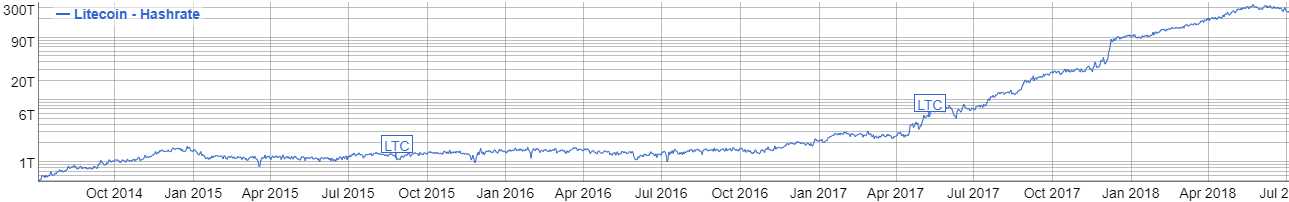
\includegraphics[width=1.0\linewidth]{provahashratelog}
	\caption{Litecoin Hashrate 2014-2018, da bitinfocharts.com}
	\label{fig:provahashratelog}
\end{figure}

\begin{figure}
	\centering
	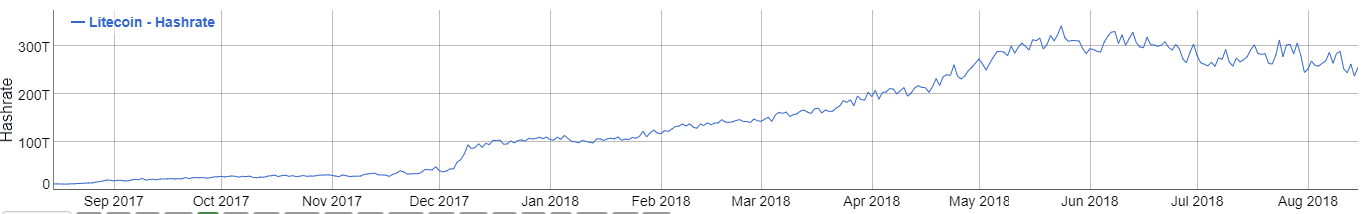
\includegraphics[width=1.0\linewidth]{LitecoinHashRateLIN}
	\caption{Litecoin Hashrate 2018 da bitinfocharts.com}
	\label{fig:litecoinhashratelin}
\end{figure}


La suddivisione riportata in seguito è datata 02/08/2018, è limitatamente indicativa nel tempo e presenta un margine d’errore di qualche punto percentuale: i dati istantanei sulla distribuzione dell’hashing power sulla rete sono molto variabili poiché l’unico modo per ottenerli sono delle stime effettuate sulla base della velocità del network nel processare i nuovi blocchi e delle indicazioni fornite dai pools stessi. Tuttavia la loro osservazione fornisce dati utili per comprendere meglio i risultati delle analisi.


\begin{figure}[h!]
	\centering
	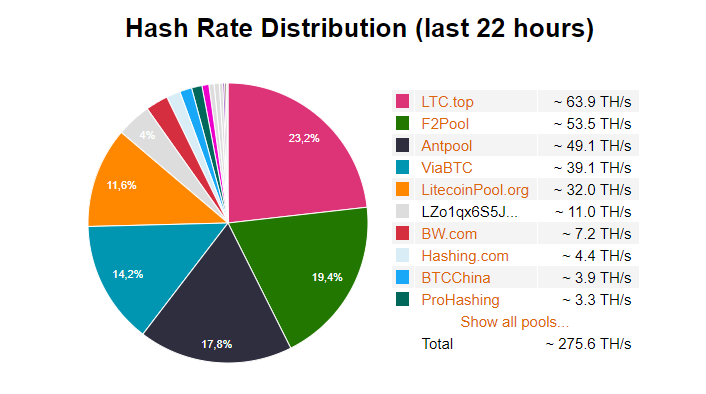
\includegraphics[width=1.0\linewidth]{images/HashingPower020818}
	\caption{dati 02/08/2018 litecoinpool.org}
	\label{fig:hashingpower020818}
\end{figure}


\subsection{Obiettivo dell’analisi}
Verificare la distribuzione del potere di mining nel tempo: ci sono pools che superano il 50\% di hashing power? Per il mantenimento della decentralizzazione della Blockchain è importante che questo non accada perché si configurerebbe il rischio di un cosiddetto 51\% attack: quando qualcuno riesce a disporre di una potenza di calcolo superiore al 50\% del totale, può creare blocchi non rispondenti alle specifiche del protocollo della criptovaluta, tra cui ad esempio blocchi contraffatti con i quali spendere due volte gli stessi token o addirittura impedire ad altri miner di validare il blocco al fine di incassare le reward.


\subsection{Svolgimento}
Ogni nuovo blocco minato contiene una transazione, detta coinbase, che non contiene alcun input ma contiene in output la somma di ricompensa per il blocco minato e fees di tutte le transazioni in esso contenute.
Spesso i mining pools inseriscono nella coinbase un identificatore come una sigla, un codice ascii o non ascii, oppure il proprio nome seguito dal miner per “firmare” il blocco. È sufficiente esaminare tramite visualizzatore esadecimale l’hex della coinbase di un blocco per verificare se è presente un identificatore di questo tipo.

Il tool BlockAPI contiene una lista di identificatori noti per Bitcoin ed Ethereum, ai quali ho aggiunto alcuni identificatori o pattern relativi a mining pools che minano Litecoin oppure sia Bitcoin che Litecoin. 
Dopo la creazione della tabella, viene eseguito il seguente script per popolarla:

\begin{lstlisting}
blockchain.foreach(block => {
txTable.insert(Seq(block.hash.toString(), convertDate(block.date), block.getMiningPool(), block.isMerged()))
})
\end{lstlisting}

Per ogni blocco nell’intervallo selezionato, si inserisce nella tabella l’hash del blocco, il timestamp, il pool che ha minato il blocco e un ulteriore campo relativo al merged mining (che tratterò nelle analisi successive). La funzione getMiningPool() fa parte dell’interfaccia Block, che in questo caso è overrided [?] da getLitecoinPool(txs.head). L’override effettuato per ogni blockchain permette di verificare per ogni criptovaluta la presenza di uno degli identificatori ad essa relativi.


\subsection{Query}

\begin{lstlisting}
SELECT Pool.pool AS Pool, COUNT(*) AS Blocks
FROM myblockchainlite.ltcpools AS Pool
GROUP BY Pool.pool
ORDER BY Blocks DESC;
\end{lstlisting}

\subsection{Risultati}

Su un totale di 312432 blocchi di cui ci è noto il miner, possiamo fare le seguenti osservazioni:

\begin{figure}[h!]
	\centering
	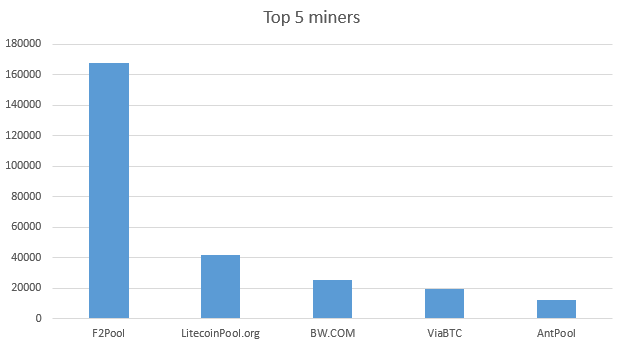
\includegraphics[width=1.0\linewidth]{images/top5miners}
	\caption{I 5 pools che hanno minato più blocchi LTC. Dati ottenuti tramite BlockAPI}
	\label{fig:top5miners}
\end{figure}


I primi 5 miners hanno complessivamente minato 265756 blocchi. Risulta quindi che l’85\% dell’hashing power dei blocchi di miner noto sia concentrato nei primi 5. 
F2Pool, noto anche come DiscusFish e attivo dal 2013 su BTC, ETH e altre criptovalute, è stato uno dei primi pools importanti ad interessarsi a Litecoin e domina totalmente il computo totale con un impressionante 53.64\% dei blocchi noti della blockchain. Correntemente ha un hashing power che si attesta intorno al 20\% del totale.

\begin{figure}[h!]
	\centering
	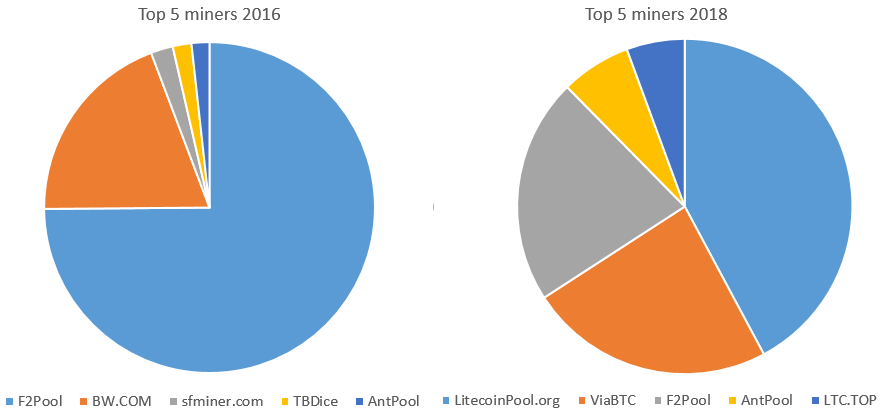
\includegraphics[width=1.0\linewidth]{images/top5miners2016vs2018}
	\caption{Distribuzione dei blocchi tra i 5 maggiori mining pools, confronto tra 2016 e 2018. Dati ottenuti tramite BlockAPI}
	\label{fig:top5miners2016vs2018}
\end{figure}



Il confronto tra i dati del 2016 e i dati (ovviamente parziali) del 2018 evidenziano il cambio di distribuzione del mining di Litecoin: se da un lato la maggior distribuzione dei blocchi minati tra i mining pools indica una migliore decentralizzazione, dall’altro evidenzia che i miners indipendenti o i piccoli pools sono praticamente scomparsi a causa dell’aumento della difficoltà, correntemente > 10.000.000.

Infatti se nel 2014 201587 blocchi risultano minati da ignoti su un totale di 215094 (93.7\%) denotando un interesse molto marginale da parte dei mining pools, perlopiù pools già operativi su Bitcoin, e molto maggiore da parte di miners privati, nel 2017 la percentuale scende al 42\% in cui va tenuto conto di margine d’errore dovuto a due cause: la prima, logica, è che potrebbero esserci dei mining pools di cui non si conoscono gli identificatori o non ne usano oppure potremmo non conoscere tutti gli identificatori di ogni mining pool tra quelli già noti, la seconda è che un bug di LitecoinJ nonché della precedente versione di BitcoinJ, sul quale al momento non è possibile intervenire, impedisce il parsing corretto dello script facendolo erroneamente risultare nullo.

A tal proposito va detto che a causa della variabilità degli identificatori utilizzati nonché del suddetto bug di LitecoinJ risulta difficile l’identificazione di alcuni blocchi, soprattutto da parte di AntPool e occasionalmente BW.COM, più di rado F2Pool, che appaiono sottodimensionati nei risultati delle mie analisi. È stato possibile effettuare delle analisi manuali sulle transazioni deserializzate per intervalli molto limitati della blockchain che confermano un’ampia presenza dei suddetti pools.

In conclusione: circa il 60\% dell’hashing power del 2017 è risultato concentrato nelle mani dei pools noti con la suddivisione in figura 3.6.

\begin{figure}[h!]
	\centering
	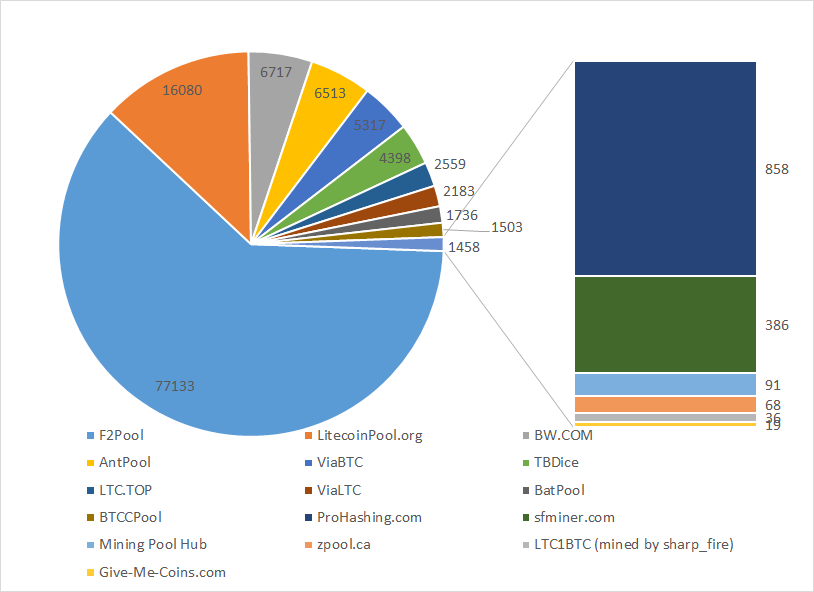
\includegraphics[width=1.0\linewidth]{images/distribuzionemining}
	\caption{blocchi per miner 2017, dati ottenuti tramite BlockAPI}
	\label{fig:distribuzionemining}
\end{figure}


\section{Merged Mining}
\subsection{Contesto}
Il merged mining, noto anche come Auxiliary Proof of Work, permette di minare contemporaneamente due criptovalute che utilizzino lo stesso algoritmo di hashing (Scrypt nel caso di Litecoin).
I calcoli vengono svolti e sfruttati per due blockchain, il che permette alle blockchain minori di aumentare il proprio potere di hashing. In questo caso il merged mining riguarda Litecoin e Dogecoin, entrambe criptovalute il cui mining è basato su Scrypt.
Ho identificato il pattern esadecimale [fabe6d6d] che viene inserito nella coinbase per segnalare che il blocco è frutto di merged mining.

\begin{figure}
	\centering
	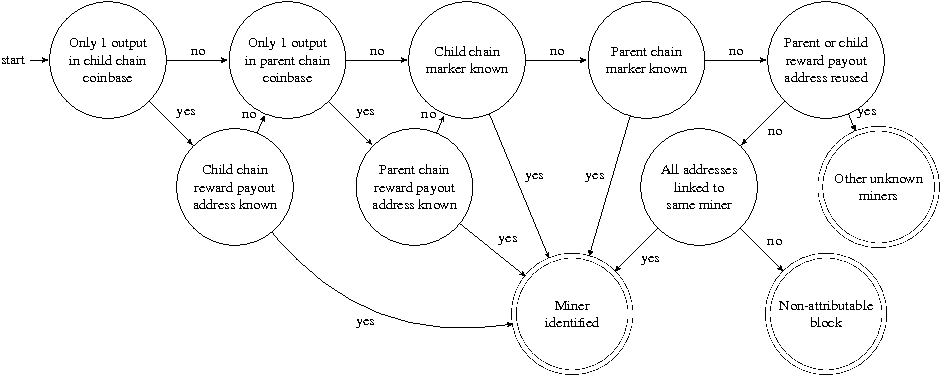
\includegraphics[width=1.0\linewidth]{images/mergedminingdiagramsemanticscholar}
	\caption{Funzionamento del merged mining, fonte Semantic Scholar}
	\label{fig:mergedminingdiagramsemanticscholar}
\end{figure}

\subsection{Obiettivo dell’analisi}
Identificare quanti blocchi vengano ottenuti tramite merged mining e chi li ha minati, la diffusione della pratica nel corso degli anni.
\subsection{Svolgimento}
L’esame dell’hex della transazione coinbase questa volta si orienterà sulla ricerca del pattern fabe6d6d. Ho effettuato l’analisi sullo stato dell’intera blockchain Litecoin fino al 02/08/2018.
\subsection{Query}

\begin{lstlisting}
SELECT COUNT(*) as "Blocks", isMerged as 'MM?' FROM myblockchainlite.ltcpools WHERE timestamp > "2018-01-01" AND pool != "unknown"
GROUP BY MM?;
\end{lstlisting}

\subsection{Risultati}


Nel 2018, 62046 blocchi su un totale di 63434 il cui pool è noto e/o rilevabile dal tool sono minati con merged mining. È il 98.37\%, da cui deduciamo che ormai la quasi totalità dei mining pools adotta questo sistema.


\begin{tabular}{|l|c|}
	\hline 
	\textbf{Year} & \textbf{MM\%} \\ 
	\hline 
	2014 & 31.29 \\ 
	\hline 
	2015 & 87.61 \\ 
	\hline 
	2016 & 98.27 \\ 
	\hline 
	2017 & 97.96 \\ 
	\hline 
	2018 & 97.82 \\ 
	\hline 
\end{tabular}
 
\begin{tabular}{|c|c|}
	\hline 
	\textbf{Blocks2018} & \textbf{MM?} \\ 
	\hline 
	1388 & No \\ 
	\hline
	62406 & Yes \\
	\hline
\end{tabular}


La figura \ref{fig:nomerged-vs-merged} mostra per ogni anno a partire dal 2014 (poiché i dati precedenti non sono significativi) la proporzione tra i blocchi frutto di merged mining e non.

\begin{figure}[h!]
	\centering
	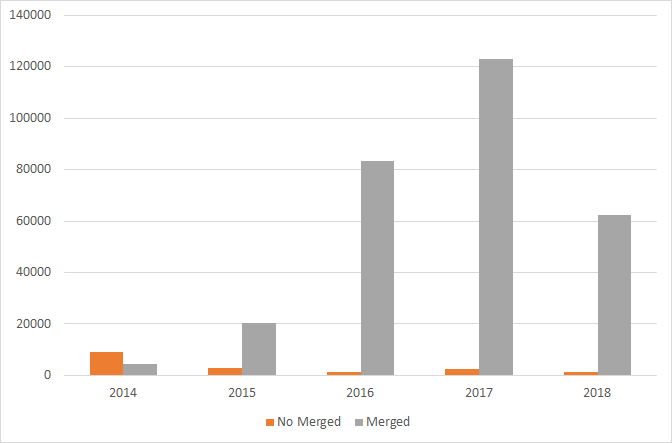
\includegraphics[width=1.0\linewidth]{images/nomerged-vs-merged}
	\caption{Proporzione tra blocchi minati con e senza merged mining. Dati ottenuti tramite BlockAPI.}
	\label{fig:nomerged-vs-merged}
\end{figure}


\section{Empty blocks}
\subsection{Contesto}
La generazione di un nuovo blocco comporta l’attribuzione della ricompensa al miner che trova la soluzione del cryptopuzzle in aggiunta alle fees, ovvero l’incentivo che l’autore di ogni transazione fornisce al miner per dare priorità all’inserimento di essa nel blocco.
Quando le fees sono trascurabili rispetto al guadagno immediato della reward, un miner (o mining pool) poco onesto può decidere di puntare unicamente alla soluzione del puzzle senza alcun impegno alla validazione delle transazioni, guadagnando così la ricompensa senza apportare nulla di utile alla blockchain. Ciò ha anche l’effetto collaterale di costringere indirettamente gli utilizzatori a ricorrere a fees più alte per fornire un incentivo ai miners per interessarsi alla transazione.
Il problema è più accentuato per le criptovalute la cui blockchain prevede una rapida generazione dei blocchi e fees mediamente basse come Litecoin.

\subsection{Obiettivo dell’analisi}
Verificare quanti blocchi vuoti vengono minati e se un particolare mining pool sta attuando sistematicamente questo comportamento.
C’è da attendersi risultati significativi da parte di mining pools con elevato hashing power.

\subsection{Svolgimento}
Ogni blocco Litecoin presenta sempre almeno una transazione coinbase, per cui si identificano i blocchi che contengono una sola transazione e chi li ha minati, se noto. Si può visualizzare, per ciascun miner, qual è il rapporto tra blocchi vuoti e non vuoti e dedurre da questo se siano casi isolati oppure segno che il pool sta attuando sistematicamente questo comportamento.

\subsection{Query}

\begin{lstlisting}
SELECT miner, COUNT(*) as emptyblocks 
FROM `emptyblockanalysis` where txsnumber = 1
GROUP BY miner
ORDER BY emptyblocks DESC;
\end{lstlisting}


Questa query conta quanti sono i blocchi vuoti minati da ciascun miner riconosciuto.

\begin{lstlisting}
SELECT miner,
COUNT(CASE WHEN txsnumber = 1 THEN 1 ELSE NULL END) AS emptyblocks,
COUNT(CASE WHEN txsnumber > 0 THEN 1 ELSE NULL END) AS totalblocks
FROM emptyblockanalysis
GROUP BY miner;
\end{lstlisting}

Tramite questa query si può confrontare il dato dell’analisi precedente, che di per sé ci dice poco, con il numero totale di blocchi che il miner in questione ha minato. Da qui possiamo evincere quali miner lo adottano come comportamento sistematico.

\begin{lstlisting}
SELECT t1.miner as BlockMiner,
t1.emptyblocks as EmptyB,
t1.totalblocks as TotalB,
t1.emptyblocks/t1.totalblocks as Ratio 
FROM ((SELECT miner,
COUNT(CASE WHEN txsnumber = 1 THEN 1 ELSE NULL END) AS emptyblocks,
COUNT(CASE WHEN txsnumber > 0 THEN 1 ELSE NULL END) AS totalblocks
FROM emptyblockanalysis
GROUP BY miner) as t1)
ORDER BY Ratio desc;
\end{lstlisting}		

Infine, questa query ci fornisce una vista ordinata in modo decrescente per ratio empty/total delineando meglio il quadro generale.				
\subsection{Risultati}

\begin{figure}[h!]
	\centering
	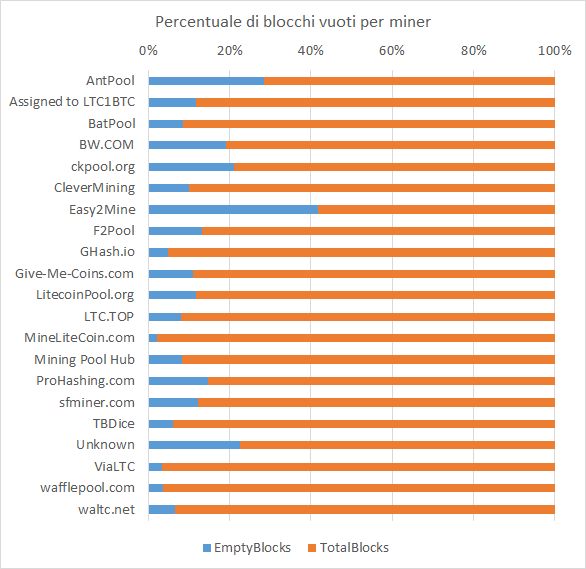
\includegraphics[width=0.8\linewidth]{images/percentuale-blocchi-vuoti-per-miner}
	\caption{\% di blocchi vuoti per i principali miners. Dati ottenuti tramite BlockAPI}
	\label{fig:percentuale-blocchi-vuoti-per-miner}
\end{figure}


Il grafico in figura \ref*{fig:percentuale-blocchi-vuoti-per-miner} indica, per ogni miner, qual è la percentuale di blocchi vuoti rispetto ai blocchi totali

Nonostante il bug citato nel cap 3.1 relativo ai mining pools che impedisce la corretta attribuzione di alcuni blocchi ai rispettivi miners, la percentuale di blocchi vuoti minati da AntPool, BW.COM e F2Pool tra quelli rilevati è visibilmente degna di nota. L’osservazione tramite un explorer esterno (nella fattispecie litecoinpool.org che sfrutta l'explorer chain.so) ha permesso di riscontrare che AntPool tende a minare anche svariati blocchi vuoti consecutivi, dimostrandosi sotto questo punto di vista uno tra i pools più negativi.
La distribuzione tra i mining pools sul totale dei blocchi vuoti riscontrati nella blockchain è riportata nella figura \ref{fig:distribuzione-blocchivuoti-ring}.

\begin{figure}[h!]
	\centering
	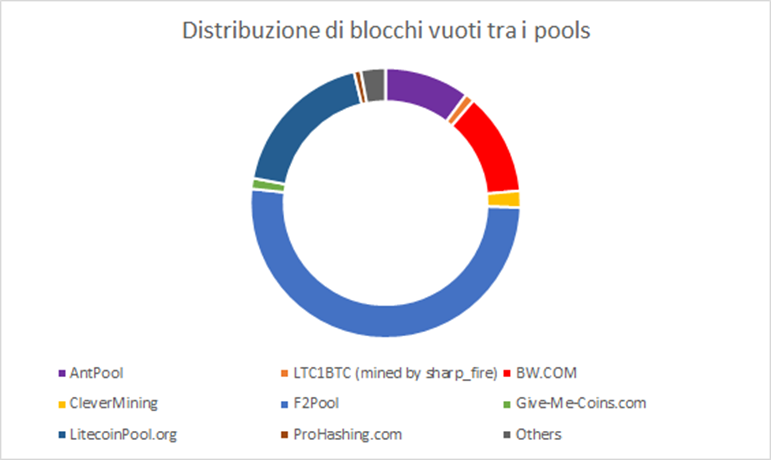
\includegraphics[width=1.0\linewidth]{images/distribuzione-blocchivuoti-ring}
	\caption{Ripartizione dei blocchi vuoti tra i pools. Dati ottenuti tramite BlockAPI}
	\label{fig:distribuzione-blocchivuoti-ring}
\end{figure}


\section{OP\_RETURN protocols}
\subsection{Contesto}
OP\_RETURN, di base, è uno degli opcodes del linguaggio Script. Rende la transazione non spendibile, per cui tutto ciò che viene inserito dopo esso non ha rilevanza e questo permette di allegare 40[80] bytes di dati arbitrari. Solitamente viene utilizzato per allegare un messaggio. Tuttavia, poiché la blockchain per ragioni di efficienza e spazio non permette l’inserimento di files allegati e la necessità di avere milioni di copie della blockchain rende impensabile l’implementazione di un servizio simile si sfrutta questo piccolo spazio per allegare in forma compatta un riferimento a dati esterni.
Tramite l’OP\_RETURN è possibile utilizzare servizi aggiuntivi che si appoggiano alla blockchain ma risiedono su un altro strato (layered network). Servizi di timestamping, firma digitale, archiviazione possono utilizzare la blockchain per includere riferimenti a dati residenti all’esterno di essa e marcare con il loro identificatore i primi 4 bytes dell’OP\_RETURN

OP\_RETURN è supportato su Litecoin a partire dalla versione 0.9: pur non avendo raggiunto una diffusione comparabile a quella conseguita su Bitcoin è stata comunque riscontrata la presenza di metaprotocolli nella blockchain, tra cui alcuni dei più noti che si appoggiano a Bitcoin stesso.
Recentemente l’OP\_RETURN è stato utilizzato per inserire un header indicativo dell’adesione a Segwit: quest’ultimo è un protocollo che nasce per ovviare ad un problema di scalabilità che riguarda la blockchain.

\begin{figure}[h!]
	\centering
	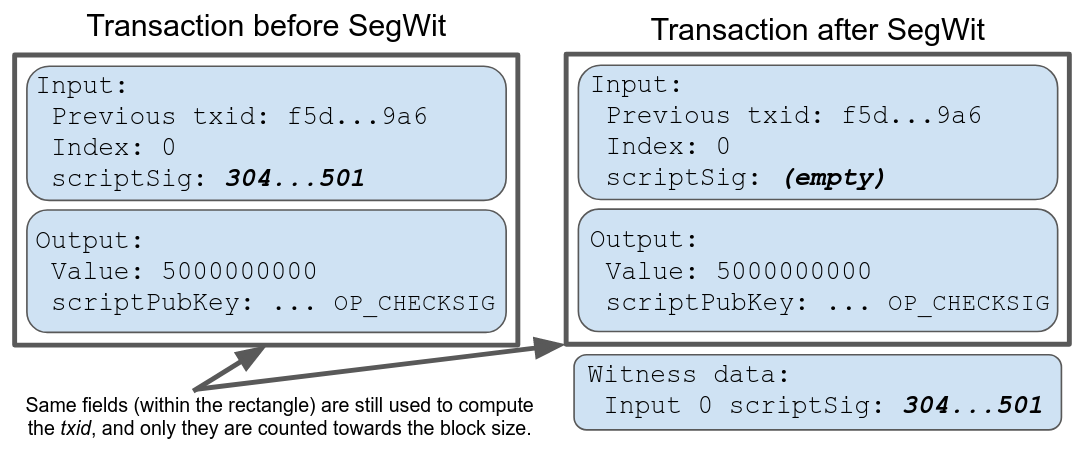
\includegraphics[width=1.0\linewidth]{images/before-after-segwit-medium}
	\caption{Transazioni prima e dopo SegWit (medium.com)}
	\label{fig:before-after-segwit-medium}
\end{figure}


Il problema si è posto con la crescita dell’interesse verso l’utilizzo delle Blockchain, in quanto ogni blocco di transazioni deve rispettare il limite massimo di 1MB e questo ha cominciato a causare congestione e ritardi sui network. Talvolta i tempi di attesa sono stati nell’ordine delle ore. Inoltre un rischio notevole per la sicurezza era rappresentato dalla malleabilità, ossia la possibilità che il destinatario intercettasse l’ID della transazione del mittente modificandola a suo favore. Queste ragioni hanno portato alla separazione (da qui Segregated) della firma digitale (Witness): i dati della firma digitale, che fino ad ora occupavano fino al 65\% dello spazio della transazione, sono ora separati e la transazione contiene un puntatore ad essi affinché il software possa trattare indipendentemente le due parti.


\begin{figure}[h]
	\centering
	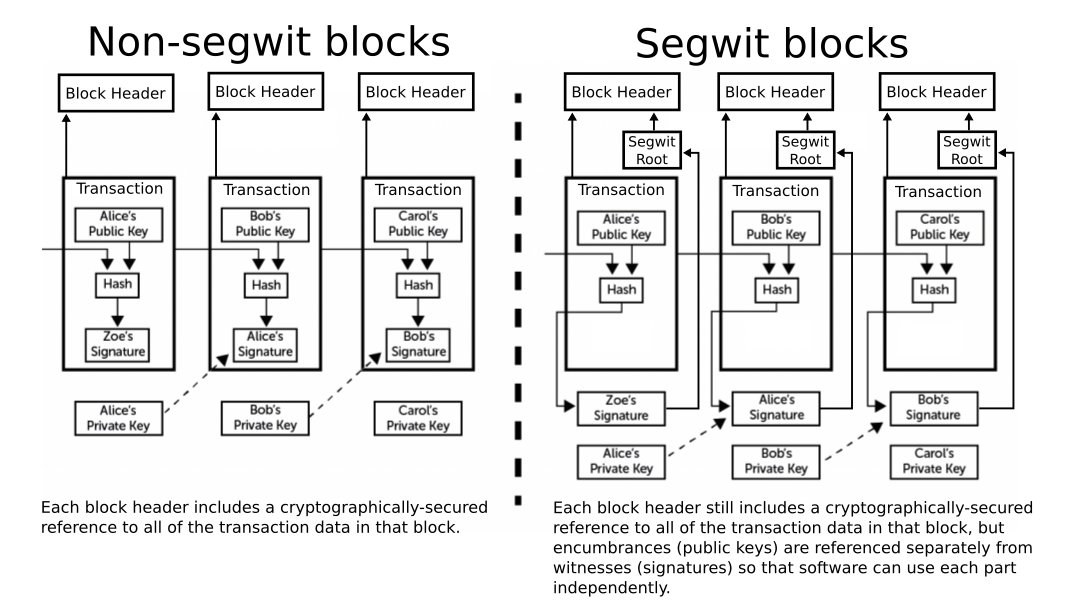
\includegraphics[width=1.0\linewidth]{images/segwitvsnonsegwit-medium}
	\caption{differenza tra blocco SegWit e non SegWit (medium.com)}
	\label{fig:segwitvsnonsegwit-medium}
\end{figure}


La condizione necessaria affinché il sistema SegWit funzioni è l’adozione da parte di almeno il 95\% del network e la segnalazione dell’adozione del sistema da parte dei miners è fondamentale per ritenere il consenso necessario all’implementazione del soft fork.


\subsection{Obiettivo}
Identificare tramite pattern noti i metaprotocolli utilizzati e l’header di adesione a SegWit.
\subsection{Svolgimento}
Si identificano le transazioni OP\_RETURN della blockchain. BlockAPI contiene una lista di pattern conosciuti utilizzati anche su Bitcoin ai quali ho aggiunto alcuni pattern scoperti tramite ricerca e consultazione dei siti ufficiali dei fornitori dei servizi.

\begin{figure}[h]
	\centering
	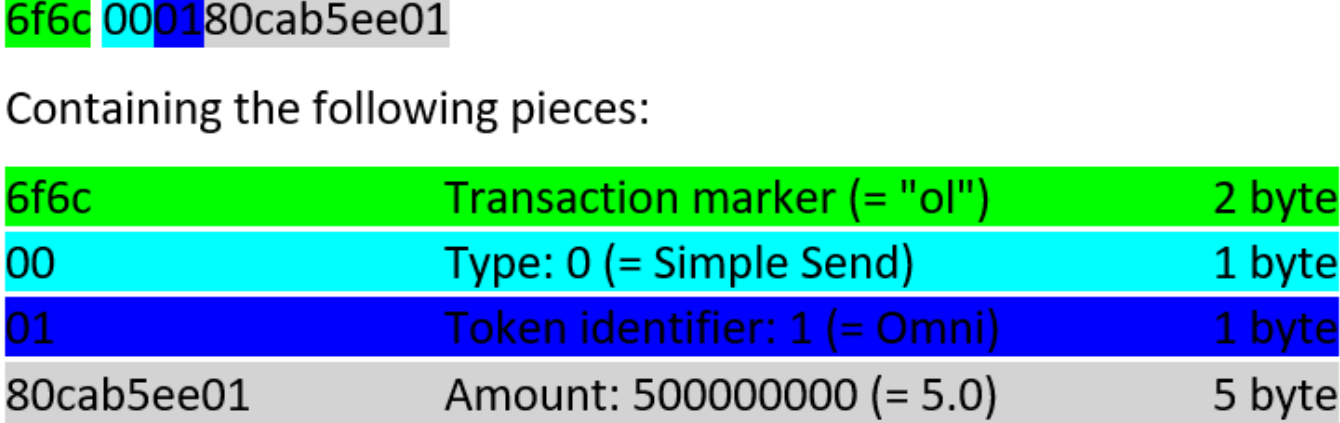
\includegraphics[width=1.0\linewidth]{images/ol-omnilayer-medium}
	\caption{Struttura di un OP\_RETURN di Omni Layer (medium.com)}
	\label{fig:ol-omnilayer-medium}
\end{figure}

Su ciascuna di esse, in modo analogo a quanto fatto sulle coinbase per l’analisi dei mining pools, si effettua un parsing dell’output tramite il seguente script:

\begin{lstlisting}
block.txs.foreach(tx => {
tx.outputs.foreach(f = out => {
if (out.isOpreturn()) {
var protocol: String =
MetadataParser.getApplication(tx.inputs.head.outPoint.toString.substring(0, 64), out.transOut.toString)
var metadata: String =
out.getMetadata()
\end{lstlisting}

Otteniamo i metadata della transazione.

\begin{lstlisting}
var segwit: Boolean =
MetadataParser.isSegwit(metadata)
\end{lstlisting}

Il Boolean ‘segwit’ restituisce true se l’OP\_RETURN rispetta la seguente struttura dichiarata sul github ufficiale:

\begin{tabular}{c|c}
	\textbf{Bytes} & \textbf{Funzione} \\ 
	\hline 
1 Byte	& OP\_RETURN (0x6A) \\ 
	\hline 
1 Byte	& Push dei seguenti 36 Bytes (0x24) \\ 
	\hline 
4 Byte	& Header SegWit (0xAA21A9ED) \\ 
	\hline 
32 Byte	& SHA256(SHA256(witness root hash|witness root value)) \\ 
	\hline 
39° e oltre	&  Dati opzionali non riguardanti il protocollo\\ 
\end{tabular} 

\begin{lstlisting}
outputTable.insert(Seq(tx.hash.toString, convertDate(block.date), protocol, metadata, segwit))
}
})
})
\end{lstlisting}
\subsection{Query}

SELECT protocol, count(*) as number FROM opreturn.opreturnoutputlite
group by protocol order by number desc;

Verifichiamo quante tra le transazioni contengono dei meta-protocolli a noi noti che si riferiscano a servizi layered.

\begin{lstlisting}
SELECT isSegwit as "Signaling Segwit?", Count(*) as TxNumber FROM opreturn.opreturnoutputlite
GROUP by isSegwit;
\end{lstlisting}

L’header della transazione “aa21a9ed” è un codice non-ascii che segnala l’utilizzo di SegWit nel blocco. Allo stato attuale dello sviluppo delle librerie di terze parti utilizzate per la blockchain Litecoin, non abbiamo a disposizione gli strumenti per effettuare ulteriori analisi sul contenuto dei metadati dell’OP\_RETURN il cui header segnali SegWit.
\subsection{Risultati}

Un primo conto significativo si può effettuare per dividere gli OP\_RETURN utilizzati allo scopo di segnalare SegWit da quelli utilizzati per qualsiasi altro scopo: come abbiamo detto è possibile utilizzarli per introdurre altri servizi esterni alla blockchain, ma anche per ancorare un messaggio in modo permanente alla blockchain seppur meno diffusamente di quanto accada su Bitcoin, nel quale la funzionalità viene sfruttata da molto più tempo.

\begin{tabular}{|c|c|}
	\hline 
	\textbf{Segwit?} & \textbf{TxCount} \\ 
	\hline 
	No & 24559 \\ 
	\hline 
	Yes & 234476 \\ 
	\hline 
\end{tabular} 

\begin{tabular}{|c|c|}
	\hline 
	\textbf{protocol}& \textbf{count}  \\ 
	\hline 
unknown	&  12381\\ 
	\hline 
copyrobo	&  7433\\ 
	\hline 
stampery	& 3577 \\ 
	\hline 
proofstack	& 967 \\ 
	\hline 
colu	& 69 \\ 
	\hline 
omni	& 67 \\ 
	\hline 
counterparty	& 35 \\ 
	\hline 
openassets	& 26 \\ 
	\hline 
blockstore	& 2 \\ 
	\hline 
empty	& 1 \\ 
	\hline 
proofofexistence	& 1 \\ 
	\hline 
\end{tabular} 

Esaminiamo ora gli OP\_RETURN utilizzati per uno scopo diverso dalla segnalazione di SegWit: approssimativamente il 50\% non denota l’utilizzo di un metaprotocollo specifico. Questo numero include OP\_RETURNs che contengono messaggi testuali, stringhe la cui decodifica non corrisponde ad alcun ascii, eventualmente codificati in base-64 o in altro modo, e infine protocolli a noi ancora non noti o di cui non è stato possibile trovare un riscontro affidabile sul web.
La diffusione dei vari protocolli nel restante 50\% è riportata nella tabella.

\begin{figure}
	\centering
	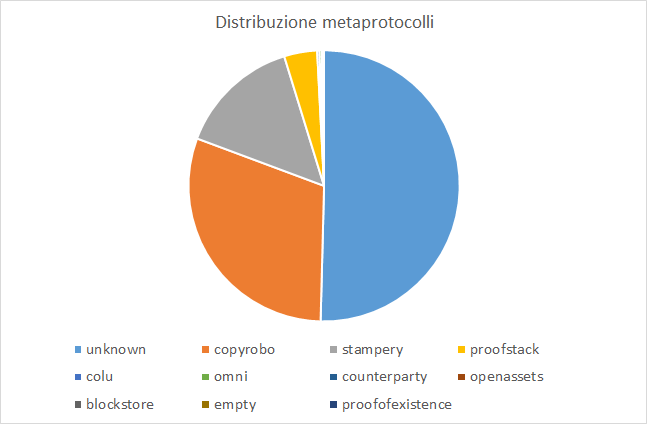
\includegraphics[width=1.0\linewidth]{images/distribuzioneopreturn}
	\caption{Ripartizione dei metaprotocolli negli op\_return della blockchain Litecoin. Dati ottenuti tramite BlockAPI}
	\label{fig:distribuzioneopreturn}
\end{figure}

